% !TeX spellcheck = en_GB
\chapter{Trivalent categories}
\label{ch:Trivalent}

In this section, we describe monoidal categories that are generated by a trivalent vertex, which is a rotationally invariant morphism in $\Hom_\C(\mathbf{1},X\otimes X\otimes X)$, where $X$ is a specific simple object in the category. These categories were presented and extensively studied in \cite{Morrison2017} and they can be thought of as fusion categories without finiteness, i.e., there can be an infinite number of simple objects. They are especially nice to work with since their graphical calculus has some additional rules that greatly simplify calculations with string diagrams. We will need a few additional adjectives before we can state the definition. Note that a trivalent category is not necessarily a fusion category or a Modular Tensor Category (MTC), although there are some examples of MTCs and fusion categories which are also trivalent categories. The latter cases are the reason why trivalent categories appear in the context of this thesis and we will discuss some examples of trivalent fusion categories in detail later. In particular, one of the Haagerup fusion categories can be described as a trivalent category, which allows us to exploit its simple graphical calculus to simplify certain calculations in \cref{ch:Haagerup}.

\section{Basic definitions}

Unless otherwise specified, all categories in this chapter are assumed to be monoidal.

	\begin{defn}[Evaluable]
		Let $k$ be a field. A $k$-linear category $\C$ is evaluable\index{evaluable category} if $\dim(\Hom(\mathbf{1},\mathbf{1}))=1$. In fact, $\Hom(\mathbf{1,\mathbf{1}})$ can be identified with the ground field $k$ of the category by sending the empty diagram to $1$.
	\end{defn}

	\begin{defn}[Nondegenerate]
		A pivotal category $\C$ is called nondegenerate\index{nondegenerate category} if for every morphism $f\in\Hom(X,Y)$ there is a morphism $f'\in\Hom(Y,X)$ such that $\Tr(f'\circ f)\neq 0\in\Hom(\mathbf{1,\mathbf{1}})$.
	\end{defn}
	
	\begin{rem}
		For a pivotal category $\C$ and an object $X$ we will use the notation
			\begin{equation}
				\mathfrak{C}_k\equiv\Hom_\C(\mathbf{1},X^{\otimes k}).
			\end{equation}
		We use the convention that $X^{\otimes 0}=\mathbf{1}$.
	\end{rem}
	
	\begin{defn}[Trivalent category]
		A trivalent category\index{trivalent category} is a tuple $(\C,X,\tau)$, where $\C$ is a nondegenerate evaluable pivotal category over $\mathbb{C}$ with an object $X$ with $\dim(\mathfrak{C}_1) = 0$, $\dim(\mathfrak{C}_2) = 1$, and $\dim(\mathfrak{C}_3) = 1$, with a rotationally invariant morphism $\tau\in\mathfrak{C}_3$ called the \emph{trivalent vertex}, such that the category is generated (as a pivotal category) by $\tau$ .
	\end{defn}

	The constraints on the dimensions of certain morphism spaces in the definition of a trivalent category can be interpreted as follows: 
		\begin{enumerate}
			\item Firstly, $\dim\mathfrak{C}_1=0$ implies that there is no map from the object $X$ to the unit. This means that $X$ is not the unit and it is not a sum that contains the unit object.
			\item The second constraint, $\dim\mathfrak{C}_2=1$ says that $X$ is simple, i.e., it is not isomorphic to the unit object and every subobject of $X$ is isomorphic to zero or $X$.
			\item The last constraint, $\dim\mathfrak{C}_3=1$, together with the rotational invariance of the trivalent vertex $\tau\in\mathfrak{C}_3$, implies that we do not need to carry any label that indicates the orientation of the trivalent vertex.
		\end{enumerate}
	
	\begin{rem}
		We can show that the object $X$ is symmetrically self-dual (see \cite[Lemma 2.2]{Morrison2017}), which allows us to omit orientations on strings. Combining these two facts, we can interpret any unoriented planar trivalent string diagram with $n$ boundary points as an element of $\mathfrak{C}_n$.
	\end{rem}

	\begin{rem}
		Any trivalent category is spherical (see \cite[Rem.\ 2.5]{Morrison2017}). Since every object of the category is generated by the simple object $X$, we only need to check that the dimension of $X$ is equal to the dimension of $X^*$, but this is obvious since $X$ is self-dual.
	\end{rem}

\subsection*{Graphical calculus of trivalent categories.} 

	We now explain the additional rules of the graphical calculus that are imposed by the definition of a trivalent category. In the course of this we will also introduce some parameters which play an important role in the classification of these categories. Most importantly, since the category is generated by the translational invariant trivalent vertex $\tau$, we do not need to put an orientation or a label on the strings in the diagrams. Every string is labelled with the object $X$ of the category. Moreover, we are allowed to deform and rotate the diagrams without changing their value. Then, there is basically one additional rule (and one parameter) that simplifies the evaluation of diagrams for each constraint on the dimensions of morphism spaces:
		\begin{enumerate}
			\item Since the category is evaluable, we know that $\dim\mathfrak{C}_0=1$. This implies that each diagram with a loop in it has to be a multiple $d$ of the same diagram without that loop:
				\begin{equation}
				\label{eq:loop}
					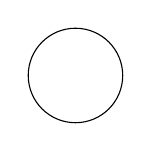
\begin{tikzpicture}[baseline=(current bounding box.center)]
						\draw (0,0) circle[radius=0.6cm];
					\end{tikzpicture}\ =d.
				\end{equation}
			Here, the parameter $d$ is a characteristic of the category. It has to be non-zero since it is the dimension of the specific simple object $X$ that generates the category. It also follows from the fact that the loop is the pairing of the unique (up to scalar) element of $\mathfrak{C}_2$ with itself, i.e.,
				\begin{equation}
					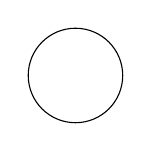
\begin{tikzpicture}[baseline=(current bounding box.center)]
					\draw (0,0) circle[radius=0.6cm];
					\end{tikzpicture}\ =\ 
					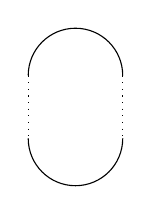
\begin{tikzpicture}[baseline=(current bounding box.center)]
						\draw (0,0) arc(0:180:0.6);
						\draw (-1.2,-0.8) arc(180:360:0.6);
						\draw[dotted] (0,0) -- (0,-0.8);
						\draw[dotted] (-1.2,0) -- (-1.2,-0.8);
					\end{tikzpicture}
				\end{equation}
			 and that the category is nondegenerate.
			 \item The constraint $\dim\mathfrak{C}_1=0$ implies that there are no diagrams with only one boundary point, i.e, ``lollipops'' are forbidden:
			 	\begin{equation}
			 	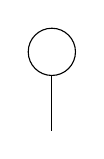
\begin{tikzpicture}[baseline=(current bounding box.center)]
			 		\draw (0,0) circle[radius=0.3cm];
			 		\draw (0,-0.3) -- (0,-1);
			 	\end{tikzpicture}\ =0.
			 	\end{equation}
			 Whenever some kind of lollipop is part of a diagram, that diagram evaluates to zero.
			 \item The constraint $\dim\mathfrak{C}_2=1$ yields a relation
			 	\begin{equation}
			 	\label{eq:bigon}
				 	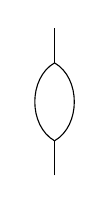
\begin{tikzpicture}[scale=1.1,baseline=(current bounding box.center)]
					 	\draw (0,-0.1) -- (0,0.3);
					 	\draw (0,0.3) to [bend left=60] (0,1.2);
					 	\draw (0,0.3) to [bend right=60] (0,1.2);
					 	\draw (0,1.2) -- (0,1.6);
				 	\end{tikzpicture}\ =\ b\cdot\ 
				 	\begin{tikzpicture}[scale=1.1,baseline=(current bounding box.center)]
				 		\draw (0,-0.1) -- (0,1.6);
				 	\end{tikzpicture}
			 	\end{equation}
			 where the parameter $b$ is again non-zero, because the diagram on the left hand side of the equation has to be non-zero with the same argument as above.
			 \item The constraint $\dim\mathfrak{C}_3=1$ yields another equation:
			 	\begin{equation}
			 	\label{eq:triangle}
				 	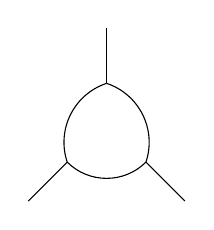
\begin{tikzpicture}[baseline=(current bounding box.center)]
					 	\draw (0.5,1) -- (0.5,1.7);
					 	\draw (0.5,1) to [bend right=45] (0,0);
					 	\draw (0.5,1) to [bend left=45] (1,0);
					 	\draw (0,0) to [bend right=45] (1,0);
					 	\draw (0,0) -- ++(225:0.7cm);
					 	\draw (1,0) -- ++(315:0.7cm);
				 	\end{tikzpicture}\ = t\cdot\ 
				 	\begin{tikzpicture}[baseline=(current bounding box.center)]
					 	\draw (0,0) -- (90:1cm);
					 	\draw (0,0) -- (225:1cm);
					 	\draw (0,0) -- (315:1cm);
				 	\end{tikzpicture}
			 	\end{equation}
			 In this case, the parameter $t$ can be zero.
		\end{enumerate}
	These relations give us three parameters to characterize the underlying category, namely $d$, $b$, and $t$. However, these three parameters are not independent of each other. One can always rescale the trivalent vertex by a constant. Because of this reason, the authors of \cite{Morrison2017} chose the normalisation $b=1$ throughout their paper. We will not choose this normalisation, but a different one due to constraints coming from the physical application later in this thesis, but for now we will just keep all three parameters.
	
	\begin{defn}
		The bilinear inner product of two trivalent graphs $f,g$ with $n$ boundary points is given by	
			\begin{equation}
				\label{eq:innerprod}
				\langle f,g\rangle=\ 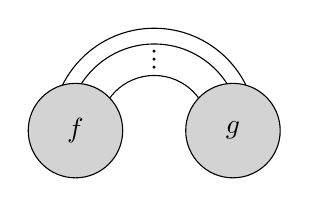
\begin{tikzpicture}[baseline=(current bounding box.center)]
					\draw (2.1,0) arc(0:180:1.1);
					\draw (2.3,0) arc(0:180:1.3);
					\draw (1.7,0) arc(0:180:0.7);
					\node[rotate=90] at (1,0.9) {$...$};
					\node [circle,draw,minimum size=1.2cm,text centered,fill=LightGray, name = f] at (0,0) {$f$};
					\node [circle,draw,minimum size=1.2cm,text centered,fill=LightGray, name = g] at (2,0) {$g$};		
				\end{tikzpicture}
			\end{equation}
		i.e., the boundary points of the diagrams are connected by $n$ strings. Since this is a diagram in $\Hom(\mathbf{1},\mathbf{1})$, the bilinear inner product is an element of $\mathbb{C}$, the ground field of the category.
	\end{defn}


\begin{exmp}[The Fibonacci category.]
	\label{ex:TrivFib}
	To illustrate the concept of a trivalent category, we consider an example which is also a modular tensor category. The Fibonacci category\index{Fibonacci category}, which we denote $\mathbf{Fib}$, has two simple objects, i.e., $\Obj(\mathbf{Fib})=\{\mathbf{1},X\}$ with the following fusion rule\footnote{Fusing an object $X$ with the unit object $\mathbf{1}$ always yields a trivial fusion rule of the form $X\otimes\mathbf{1}=X$, therefore we usually do not list these kind of fusion rules.}:
		\begin{align}
			X\otimes X&=\mathbf{1}+X.
		\end{align}
	This implies that $X$ is the generating object of the trivalent category and the corresponding trivalent vertex $\tau$ is
		\begin{equation}
			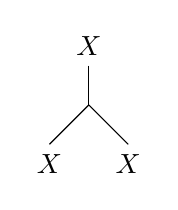
\begin{tikzpicture}[baseline=(current bounding box.center)]
				\draw (0,-0.5) -- (0,-1);
				\draw (0,-1) -- (-0.5,-1.5);
				\draw (0,-1) -- (0.5,-1.5);
				\node at (0,-0.5)[above] {$X$};
				\node at (0.5,-1.5)[below] {$X$};
				\node at (-0.5,-1.5)[below] {$X$};
			\end{tikzpicture}
		\end{equation}
	The characteristic parameters for $\mathbf{Fib}$ are given by
		\begin{equation}
			d^2=d+1,\hspace{30pt}b=1,\hspace{30pt}t=\frac{d-2}{d-1}.
		\end{equation}
	The equation for the parameter $d$ allows two solutions, namely the golden ration $\frac{1+\sqrt{5}}{2}$ and its Galois conjugate, $\frac{1-\sqrt{5}}{2}$. This is one of the reasons why this category is called Fibonacci category. The other reason is because the dimensions of the morphism spaces, $\mathfrak{C}_n$, are given by the Fibonacci series:
		\begin{table}[H]
			\centering
			\begin{tabular}{c|c}
				$n$ & $\dim(\mathfrak{C}_n)$\\ \hline \\[-0.3cm]
				$0$ & $1$\\
				$1$ & $0$\\
				$2$ & $1$\\
				$3$ & $1$\\
				$4$ & $2$\\
				$5$ & $3$\\
				$6$ & $5$\\
				$\dots$ & $\dots$
			\end{tabular}
		\end{table}
	\noindent
	The dimensions of the morphism spaces $\mathfrak{C}_0,\dots,\mathfrak{C}_3$ fulfil the constraints given by the definition of a trivalent category. The dimension of the next morphism space, however, yields an additional equation for the graphical calculus. Note that there are exactly four diagrams in $\mathfrak{C}C_4$ without internal faces, namely 
		\begin{equation}
		\label{eq:C4diags}
			\Cfourone,\hspace{10pt}
			\Cfourtwo,\hspace{10pt}
			\Cfourthree,\hspace{10pt}
			\Cfourfour.
		\end{equation}
	Since the dimension of the morphism space $\mathfrak{C}_4$ is $2$, we find the following two relations between these diagrams (see \cite{Morrison2017}):
		\begin{equation}
		\label{eq:dimC43}
			\Cfourfour-\Cfourthree+\frac{1}{d+1}\ \Cfourone+\frac{1}{d-1}\ \Cfourtwo=0,
		\end{equation}
		\begin{equation}
		\label{eq:dimC42}
			\Cfourone-\frac{1}{d}\ \Cfourtwo=\Cfourthree.
		\end{equation}
	The first equation is in fact true for all trivalent categories with $\dim(\mathfrak{C}_4)\le 3$, while the second equation is a consequence of $\dim(\mathfrak{C}_4)\le 2$ which only holds for the Fibonacci category.
\end{exmp}


\section{Cubic trivalent categories} 
\label{sec:cubictriv}

We will now look into more detail at the classification of so-called \emph{cubic} categories. These are categories where, in addition to the properties of a trivalent category, $\dim(\mathfrak{C}_4)=4$. This implies that there are no relations of the form \cref{eq:dimC43} or \cref{eq:dimC42}, since every diagram listed in \cref{eq:C4diags} is a basis element.

	\begin{defn}[Cubic category]
		A trivalent category $(\C,X,\tau)$ is called cubic\index{cubic category} if $\dim(\mathfrak{C}_4)=4$.
	\end{defn}

In a cubic category, the elements listed in \cref{eq:C4diags} form a basis of $\mathfrak{C}_4$ (this is shown in \cite[Proposition 4.16]{Morrison2017}). However, these are not the only diagrams in $\mathfrak{C}_4$. It is also possible to have diagrams with internal faces, for example
	\begin{equation}
	\label{eq:square}
		\begin{tikzpicture}[baseline=(current bounding box.center)]
			\draw (0,0) rectangle (1,1);
			\draw (0,0) -- (-0.3,-0.3);
			\draw (0,1) -- (-0.3,1.3);
			\draw (1,0) -- (1.3,-0.3);
			\draw (1,1) -- (1.3,1.3);
		\end{tikzpicture}\ .
	\end{equation}
With the rules we have listed so far, we are unable to evaluate these kinds of diagrams, but since it is not a basis element there has to be a decomposition of the above diagram in terms of the basis elements. In \cite{Morrison2017}, this calculation was only done in the case $b=1$. We will need the general case $b\neq 1$ later in this thesis, therefore we calculate the general expression in the following. 

To calculate relations between diagrams in $\mathfrak{C}_4$, we need an orthonormal basis of this space. We know that the diagrams in \cref{eq:C4diags} form a basis of $\mathfrak{C}_4$, hence we can use them do do Gram-Schmidt orthonormalisation. We label the diagrams in the following way:
	\begin{alignat}{2}
		w_1&=\Cfourone\hspace{30pt} w_2&&=\Cfourtwo\\
		w_3&=\Cfourthree\hspace{30pt} w_4&&=\Cfourfour
	\end{alignat}
Using the Gram-Schmidt orthonormalisation algorithm we can find a matrix $\Theta$ such that the orthonormal basis vectors $v_i$ are of the form
	\begin{equation}
		v_i=\sum_k\Theta_{ik} w_k.
	\end{equation}
The matrix $\Theta$ is of the form
	\begin{equation}
		\Theta=
		\begin{pmatrix}
		\frac{1}{|d|} & 0 & 0 & 0 \\
		-\frac{1}{d\sqrt{d^2-1}} & \frac{1}{\sqrt{d^2-1}} & 0 & 0 \\
		-\frac{\mathrm{sgn}(b) \sqrt{d}}{\sqrt{(d^2-a)(d^2-d-1)}} & \frac{\mathrm{sgn}(b)}{\sqrt{(d^2-a)(d^2-d-1)}} & \sqrt{\frac{d^2-1}{b^2d(d^2-d-1)}} & 0 \\
		\frac{b+dt}{d^2-d-1} C_\Theta & \frac{b-bd-t}{d^2-d-1} C_\Theta & \frac{-d^2t+t-b}{b(d^2-d-1)} C_\Theta & C_\Theta
		\end{pmatrix}
	\end{equation}
with
	\begin{equation}
		C_\Theta=\sqrt{\frac{d^2-d-1}{d(b^2d(d-2)-2bt-(d^2-1)t^2}}\ .
	\end{equation}
Using this orthonormal basis, we can write the square diagram \cref{eq:square} (which we will denote $w_\mathrm{sq}$) as a linear combination of the $v_i$:
	\begin{align}
		w_\mathrm{sq}&=\sum_i c_i v_i\\
		&= \sum_i \langle  v_i,w_{\mathrm{sq}} \rangle\ v_i
	\end{align}
with the inner product described in \cref{eq:innerprod}. In terms of the (non-orthonormal) basis diagrams given in \cref{eq:C4diags}, this has the form
	\begin{equation}
	\label{eq:squarelincom}
		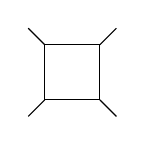
\begin{tikzpicture}[scale=0.7,baseline={([yshift=-3pt]current bounding box.center)}]
		\draw (0,0) rectangle (1,1);
		\draw (0,0) -- (-0.3,-0.3);
		\draw (0,1) -- (-0.3,1.3);
		\draw (1,0) -- (1.3,-0.3);
		\draw (1,1) -- (1.3,1.3);
		\end{tikzpicture}=\underbrace{\frac{b(b^2+bt-t^2)}{bd+t+dt}}_{\equiv \alpha}\left(\ 
		\Cfourone+
		\Cfourtwo\ \right)
		+\underbrace{\frac{t^2(d+1)-b^2}{bd+t+dt}}_{\equiv\beta}\left(\ 
		\Cfourthree+
		\Cfourfour\ \right).
	\end{equation}
In this fashion, all diagrams in $\mathfrak{C}_4$ with an arbitrary number of internal faces can be expressed as a linear combination of basis diagrams. This especially equips us with the techniques we need to evaluate any diagram in $\mathfrak{C}_0$ that includes arbitrarily many faces with four edges. Consider for example the following diagram:
	\begin{equation}
		\begin{tikzpicture}[scale=0.9,baseline=(current bounding box.center)]
			\draw[LinkColor] (0,0) rectangle (1,1);
			\draw[LinkColor] (0,0) -- (-0.3,-0.3);
			\draw[LinkColor] (0,1) -- (-0.3,1.3);
			\draw[LinkColor] (1,0) -- (1.3,-0.3);
			\draw[LinkColor] (1,1) -- (1.3,1.3);
			\draw (-0.3,-0.3) to (-0.3,1.3) to (1.3,1.3) to (1.3,-0.3) to (-0.3,-0.3);
		\end{tikzpicture}
	\end{equation}
The inner (red) part of the diagram is exactly the diagram we have expressed in terms of basis elements in \cref{eq:squarelincom}, hence we can insert this relation into the diagram and compute its value:
	\begin{align}
		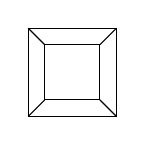
\begin{tikzpicture}[scale=0.7,baseline={([yshift=-3pt]current bounding box.center)}]
		\draw (0,0) rectangle (1,1);
		\draw (0,0) -- (-0.3,-0.3);
		\draw (0,1) -- (-0.3,1.3);
		\draw (1,0) -- (1.3,-0.3);
		\draw (1,1) -- (1.3,1.3);
		\draw (-0.3,-0.3) to (-0.3,1.3) to (1.3,1.3) to (1.3,-0.3) to (-0.3,-0.3);
		\end{tikzpicture}&=
		\alpha\left(\ 
		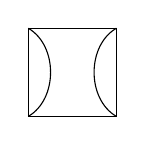
\begin{tikzpicture}[scale=0.7,baseline={([yshift=-3pt]current bounding box.center)}]
		\draw (-0.3,-0.3) to [bend right=60] (-0.3,1.3);
		\draw (1.3,-0.3) to [bend left=60] (1.3,1.3);
		\draw (-0.3,-0.3) to (-0.3,1.3) to (1.3,1.3) to (1.3,-0.3) to (-0.3,-0.3);
		\end{tikzpicture}+
		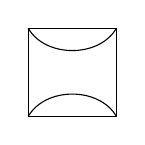
\begin{tikzpicture}[scale=0.7,baseline={([yshift=-3pt]current bounding box.center)}]
		\draw (-0.3,-0.3) to [bend left=60] (1.3,-0.3);
		\draw (-0.3,1.3) to [bend right=60] (1.3,1.3);
		\draw (-0.3,-0.3) to (-0.3,1.3) to (1.3,1.3) to (1.3,-0.3) to (-0.3,-0.3);
		\end{tikzpicture}\ \right)
		+\beta\left(\ 
		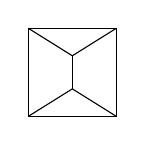
\begin{tikzpicture}[scale=0.7,baseline={([yshift=-3pt]current bounding box.center)}]
		\draw (-0.3,-0.3) to (0.5,0.2) to (1.3,-0.3);
		\draw (-0.3,1.3) to (0.5,0.8) to (1.3,1.3);
		\draw (0.5,0.2) to (0.5,0.8);
		\draw (-0.3,-0.3) to (-0.3,1.3) to (1.3,1.3) to (1.3,-0.3) to (-0.3,-0.3);
		\end{tikzpicture}+
		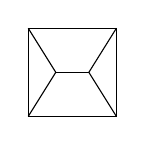
\begin{tikzpicture}[scale=0.7,baseline={([yshift=-3pt]current bounding box.center)}]
		\draw (-0.3,-0.3) to (0.2,0.5) to (-0.3,1.3);
		\draw (1.3,-0.3) to (0.8,0.5) to (1.3,1.3);
		\draw (0.2,0.5) to (0.8,0.5);
		\draw (-0.3,-0.3) to (-0.3,1.3) to (1.3,1.3) to (1.3,-0.3) to (-0.3,-0.3);
		\end{tikzpicture}\ \right)\\
		&=
		\alpha\left(\ b^2\ 
		\begin{tikzpicture}[scale=0.7,baseline={([yshift=-3pt]current bounding box.center)}]
		\draw (-0.3,-0.3) to (-0.3,1.3) to (1.3,1.3) to (1.3,-0.3) to (-0.3,-0.3);
		\end{tikzpicture}+b^2\ 
		\begin{tikzpicture}[scale=0.7,baseline={([yshift=-3pt]current bounding box.center)}]
		\draw (-0.3,-0.3) to (-0.3,1.3) to (1.3,1.3) to (1.3,-0.3) to (-0.3,-0.3);
		\end{tikzpicture}\ \right)
		+\beta\left(\ t^2\ 
		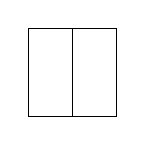
\begin{tikzpicture}[scale=0.7,baseline={([yshift=-3pt]current bounding box.center)}]
		\draw (0.5,-0.3) to (0.5,1.3);
		\draw (-0.3,-0.3) to (-0.3,1.3) to (1.3,1.3) to (1.3,-0.3) to (-0.3,-0.3);
		\end{tikzpicture}+t^2\ 
		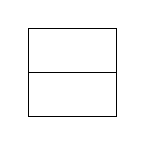
\begin{tikzpicture}[scale=0.7,baseline={([yshift=-3pt]current bounding box.center)}]
		\draw (-0.3,0.5) to (1.3,0.5);
		\draw (-0.3,-0.3) to (-0.3,1.3) to (1.3,1.3) to (1.3,-0.3) to (-0.3,-0.3);
		\end{tikzpicture}\ \right)\\
		&=
		\alpha\left(b^2 d +b^2 d\right)
		+\beta\left(t^2 bd+t^2 bd\right).
	\end{align}
In the second step, we have used the relation for bigons from \cref{eq:bigon} and the one for triangles from \cref{eq:triangle}. In the last step, we have used the loop relation \cref{eq:loop} and again the bigon relation. In this fashion we can assign to every diagram in $\mathfrak{C}_0$ an element of $\mathbb{C}$, as long as there are enough relations among the different diagrams.
	
\section{The trivalent category $\Hd$}
\label{sec:H3triv}

	We will now introduce the most important example of a category for this thesis, the Haagerup $\mathcal{H}_3$ category\index{trivalent H3@trivalent $\Hd$}, in its trivalent form. The trivalent version of the category is only a subcategory of the full $\mathcal{H}_3$ category, but it already covers a lot of the important properties that we will need throughout this thesis. Especially helpful is the graphical calculus of trivalent categories, since it can be used make statements about parts of the full category. We will see how this works in later chapters.
	
	Note that although the trivalent category is only a subcategory, the full category can be recovered from its trivalent version via the Karoubi envelope (also called the idempotent completion, see for example \cite{Morrison2010} for a detailed explanation of this technique).
	
	The trivalent category $\Hd$ is a cubic category which is characterized by the parameters
		\begin{equation}
			d=\frac{3+\sqrt{13}}{2},\hspace{30pt}b=1,\hspace{30pt}t=-\frac{2}{3}d+\frac{5}{3}.
		\end{equation} 
	Moreover, it has morphism space dimensions $\dim(\mathfrak{C}_5)=11$ and $\dim(\mathfrak{C}_6)=37$. In \cref{sec:cubictriv}, we have already seen a basis for $\mathfrak{C}_4$ and have even constructed an orthonormal basis for this space. As the dimensions of the morphism spaces increase strongly as the number of boundary points increases, doing Gram-Schmidt orthonormalisation soon becomes infeasible. However, we will see later that, when considering the full category, there is a canonical choice of orthonormal basis vectors called the \emph{fusion basis} which is much easier to construct. Therefore, we will only describe non-orthonormal bases for $\mathfrak{C}_5$ and $\mathfrak{C}_6$ in the following.
	
	There are exactly $10$ diagrams with five boundary points in $\mathfrak{C}_5$ that do not contain any faces (to distinguish different diagrams more easily we have added a dotted line around individual diagrams):
		\begin{table}[H]
			\begin{tabular}{ccccc}
				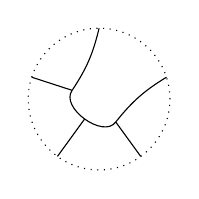
\begin{tikzpicture}[scale=0.9,baseline=(current bounding box.center)]
%				\node (A) at (90:1cm) {A};
%				\node (B) at (162:1cm) {B};
%				\node (C) at (234:1cm) {C};
%				\node (D) at (306:1cm) {D};
%				\node (E) at (18:1cm) {E};
				\draw[dotted] (0,0) circle(1cm);
				\draw (90:1cm) to [bend left=10] (162:0.4cm);
				\draw (18:1cm) to [bend right=10] (306:0.4cm);
				\draw (162:0.4cm) to [bend right=90] (306:0.4cm);
				\draw (306:0.4cm) -- (306:1cm);
				\draw (162:0.4cm) -- (162:1cm);
				\draw (234:0.35cm) -- (234:1cm);
				\end{tikzpicture} &
				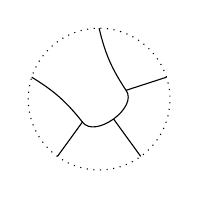
\begin{tikzpicture}[scale=0.9,baseline=(current bounding box.center)]
				\rotatebox[origin=c]{72}{
				\draw[dotted] (0,0) circle(1cm);
				\draw (90:1cm) to [bend left=10] (162:0.4cm);
				\draw (18:1cm) to [bend right=10] (306:0.4cm);
				\draw (162:0.4cm) to [bend right=90] (306:0.4cm);
				\draw (306:0.4cm) -- (306:1cm);
				\draw (162:0.4cm) -- (162:1cm);
				\draw (234:0.35cm) -- (234:1cm);}
				\end{tikzpicture} &
				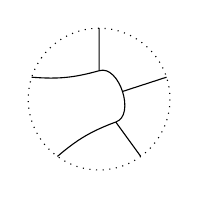
\begin{tikzpicture}[scale=0.9,baseline=(current bounding box.center)]
				\rotatebox[origin=c]{144}{
				\draw[dotted] (0,0) circle(1cm);
				\draw (90:1cm) to [bend left=10] (162:0.4cm);
				\draw (18:1cm) to [bend right=10] (306:0.4cm);
				\draw (162:0.4cm) to [bend right=90] (306:0.4cm);
				\draw (306:0.4cm) -- (306:1cm);
				\draw (162:0.4cm) -- (162:1cm);
				\draw (234:0.35cm) -- (234:1cm);}
				\end{tikzpicture} &
				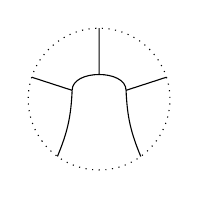
\begin{tikzpicture}[scale=0.9,baseline=(current bounding box.center)]
				\rotatebox[origin=c]{216}{
				\draw[dotted] (0,0) circle(1cm);
				\draw (90:1cm) to [bend left=10] (162:0.4cm);
				\draw (18:1cm) to [bend right=10] (306:0.4cm);
				\draw (162:0.4cm) to [bend right=90] (306:0.4cm);
				\draw (306:0.4cm) -- (306:1cm);
				\draw (162:0.4cm) -- (162:1cm);
				\draw (234:0.35cm) -- (234:1cm);}
				\end{tikzpicture} &
				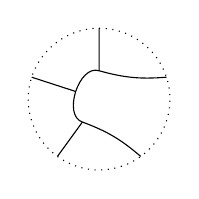
\begin{tikzpicture}[scale=0.9,baseline=(current bounding box.center)]
				\rotatebox[origin=c]{288}{
				\draw[dotted] (0,0) circle(1cm);
				\draw (90:1cm) to [bend left=10] (162:0.4cm);
				\draw (18:1cm) to [bend right=10] (306:0.4cm);
				\draw (162:0.4cm) to [bend right=90] (306:0.4cm);
				\draw (306:0.4cm) -- (306:1cm);
				\draw (162:0.4cm) -- (162:1cm);
				\draw (234:0.35cm) -- (234:1cm);}
				\end{tikzpicture}\\[1.2cm]
				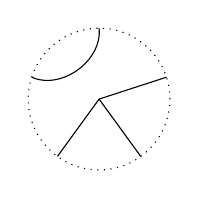
\begin{tikzpicture}[scale=0.9,baseline=(current bounding box.center)]
				\draw[dotted] (0,0) circle(1cm);
				\draw (90:1cm) to [bend left=60] (162:1cm);
				\draw (234:1cm) -- (0,0);
				\draw (306:1cm) -- (0,0);
				\draw (18:1cm) -- (0,0);
				\end{tikzpicture} &
				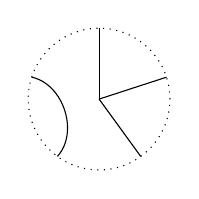
\begin{tikzpicture}[scale=0.9,baseline=(current bounding box.center)]
				\draw[dotted] (0,0) circle(1cm);
				\draw (162:1cm) to [bend left=60] (234:1cm);
				\draw (90:1cm) -- (0,0);
				\draw (306:1cm) -- (0,0);
				\draw (18:1cm) -- (0,0);
				\end{tikzpicture} &
				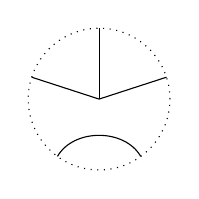
\begin{tikzpicture}[scale=0.9,baseline=(current bounding box.center)]
				\draw[dotted] (0,0) circle(1cm);
				\draw (234:1cm) to [bend left=60] (306:1cm);
				\draw (90:1cm) -- (0,0);
				\draw (162:1cm) -- (0,0);
				\draw (18:1cm) -- (0,0);
				\end{tikzpicture} &
				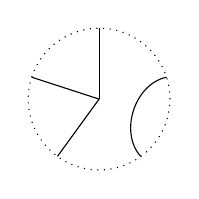
\begin{tikzpicture}[scale=0.9,baseline=(current bounding box.center)]
				\draw[dotted] (0,0) circle(1cm);
				\draw (306:1cm) to [bend left=60] (18:1cm);
				\draw (90:1cm) -- (0,0);
				\draw (162:1cm) -- (0,0);
				\draw (234:1cm) -- (0,0);
				\end{tikzpicture} &
				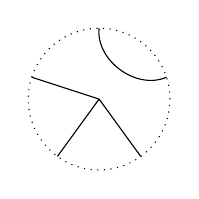
\begin{tikzpicture}[scale=0.9,baseline=(current bounding box.center)]
				\draw[dotted] (0,0) circle(1cm);
				\draw (18:1cm) to [bend left=60] (90:1cm);
				\draw (306:1cm) -- (0,0);
				\draw (162:1cm) -- (0,0);
				\draw (234:1cm) -- (0,0);
				\end{tikzpicture}
			\end{tabular}
		\end{table}
	\noindent
	and, additionally, one element with exactly one face of five edges\footnote{Note that we only take into account faces with five or more edges since in a cubic category, every face with four or less edges can be immediately removed by the relations \cref{eq:loop,eq:bigon,eq:triangle,eq:squarelincom}.}:
		\begin{equation}
			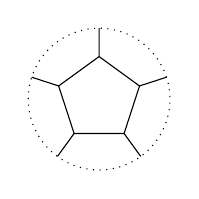
\begin{tikzpicture}[scale=0.9]
				\rotatebox{18}{
				\draw[dotted] (0,0) circle(1cm);
				\draw (0:0.6cm) -- (72:0.6cm) -- (144:0.6cm) -- (216:0.6cm) -- (288:0.6cm) -- cycle;
				\draw (0:0.6cm) -- (0:1cm);
				\draw (72:0.6cm) -- (72:1cm);
				\draw (144:0.6cm) -- (144:1cm);
				\draw (216:0.6cm) -- (216:1cm);
				\draw (288:0.6cm) -- (288:1cm);}
			\end{tikzpicture}
		\end{equation}
	Since in $\Hd$ we have $\dim(\mathfrak{C}_5)=11$, the diagrams listed above form a (non-orthonormal) basis of $\mathfrak{C}_5$ (see \cite[Proposition 7.5]{Morrison2017}). The fact that this basis is not an orthonormal one (not even an orthogonal one) can easily be seen by calculating inner products of the basis vectors. For instance, consider the inner product of the first and the sixth element of the list\footnote{The evaluation of this diagram only requires the rules of the graphical calculus \cref{eq:triangle}, \cref{eq:bigon}, and \cref{eq:loop} (in this order) and the fact that diagrams in $\mathfrak{C}_0$ can be rotated and deformed without changing their value.}:
		\begin{equation}
			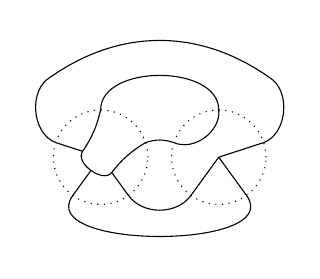
\begin{tikzpicture}[scale=0.6,baseline={([yshift=-3pt]current bounding box.center)}]
			\draw[dotted] (0,0) circle(1cm);
			\draw (90:1cm) to [bend left=10] (162:0.4cm);
			\draw (18:1cm) to [bend right=10] (306:0.4cm);
			\draw (162:0.4cm) to [bend right=90] (306:0.4cm);
			\draw (306:0.4cm) -- (306:1cm);
			\draw (162:0.4cm) -- (162:1cm);
			\draw (234:0.35cm) -- (234:1cm);
			\draw (306:1cm) to [bend right=54] ([xshift=2.5cm]234:1cm);
			\draw (234:1cm) to [bend right=126] ([xshift=2.5cm]306:1cm);
			\draw (18:1cm) to [bend left=18] ([xshift=2.5cm]162:1cm);
			\draw (90:1cm) to [bend left=90] ([xshift=2.5cm]90:1cm);
			\draw (122:2cm) to [bend left=35] ([xshift=2.5cm]58:2cm);
			\draw (162:1cm) to [bend left=65] (122:2cm);
			\draw ([xshift=2.5cm]18:1cm) to [bend right=65] ([xshift=2.5cm]58:2cm);
			\begin{scope}[shift={(2.5,0)}]
				\draw[dotted] (0,0) circle(1cm);
				\draw (90:1cm) to [bend left=60] (162:1cm);
				\draw (234:1cm) -- (0,0);
				\draw (306:1cm) -- (0,0);
				\draw (18:1cm) -- (0,0);
			\end{scope}
			\end{tikzpicture}=t b d.
		\end{equation}
	
	Finding a basis in $\mathfrak{C}_6$ is a bit more complicated, because we have to take into account a lot more diagrams since $\dim(\mathfrak{C}_6)=37$. We begin as above by finding all diagrams without faces, which are $34$ in total:
		\begin{table}[H]
			\begin{tabular}{ccc}
				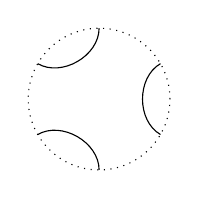
\begin{tikzpicture}[scale=0.9,baseline={([yshift=-3pt]current bounding box.center)}]
					\draw[dotted] (0,0) circle(1.cm);
%					\shade[ball color = gray!90, opacity = 0.8] (90:1.05cm) circle (0.05cm);
%					\draw (90:1.05cm) circle (0.05cm);
%					\shade[ball color = gray!90, opacity = 0.8] (150:1.05cm) circle (0.05cm);
%					\draw (150:1.05cm) circle (0.05cm);
					\draw (90:1cm) to [bend left=60] (150:1cm);
					\draw (210:1cm) to [bend left=60] (270:1cm);
					\draw (330:1cm) to [bend left=60] (30:1cm);
				\end{tikzpicture}\ +\ 1\text{ rotation,} & 
				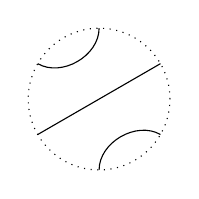
\begin{tikzpicture}[scale=0.9,baseline={([yshift=-3pt]current bounding box.center)}]
					\draw[dotted] (0,0) circle(1cm);
					\draw (90:1cm) to [bend left=60] (150:1cm);
					\draw (210:1cm) to (30:1cm);
					\draw (270:1cm) to [bend left=60] (330:1cm);
				\end{tikzpicture}\ +\ 2\text{ rotations,} &
				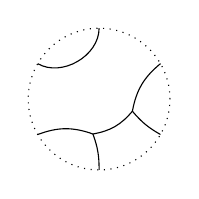
\begin{tikzpicture}[scale=0.9,baseline={([yshift=-3pt]current bounding box.center)}]
					\draw[dotted] (0,0) circle(1cm);
					\draw (90:1cm) to [bend left=60] (150:1cm);
					\draw (270:1cm) to [bend right=10] (260:0.5cm);
					\draw (330:1cm) to [bend left=10] (340:0.5cm);
					\draw (210:1cm) to [bend left=20] (260:0.5cm);
					\draw (30:1cm) to [bend right=20] (340:0.5cm);
					\draw (260:0.5) to [bend right=20] (340:0.5cm);
				\end{tikzpicture}\ +\ 5\text{ rotations,}\\[1.2cm]
				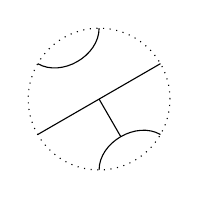
\begin{tikzpicture}[scale=0.9,baseline={([yshift=-3pt]current bounding box.center)}]
					\draw[dotted] (0,0) circle(1cm);
					\draw (90:1cm) to [bend left=60] (150:1cm);
					\draw (210:1cm) to (30:1cm);
					\draw (0,0) to (300:0.61cm);
					\draw (270:1cm) to [bend left=60] (330:1cm);
				\end{tikzpicture}\ +\ 5\text{ rotations,} &
				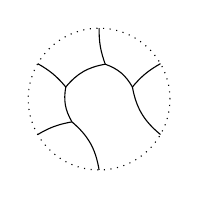
\begin{tikzpicture}[scale=0.9,baseline={([yshift=-3pt]current bounding box.center)}]
					\draw[dotted] (0,0) circle(1cm);
					\draw (90:1cm) to [bend right=10] (80:0.5cm);
					\draw (150:1cm) to [bend left=10] (160:0.5cm);
					\draw (30:1cm) to [bend right=10] (20:0.5cm);
					\draw (210:1cm) to [bend left=10] (220:0.5cm);
					\draw (270:1cm) to [bend right=20] (220:0.5cm);
					\draw (220:0.5cm) to [bend left=20] (160:0.5cm);
					\draw (160:0.5cm) to [bend left=20] (80:0.5cm);
					\draw (80:0.5cm) to [bend left=20] (20:0.5cm);
					\draw (330:1cm) to [bend left=20] (20:0.5cm);
				\end{tikzpicture}\ +\ 5\text{ rotations,} &
				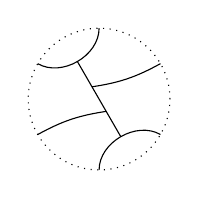
\begin{tikzpicture}[scale=0.9,baseline={([yshift=-3pt]current bounding box.center)}]
					\draw[dotted] (0,0) circle(1cm);
					\draw (90:1cm) to [bend left=60] (150:1cm);
					\draw (210:1cm) to [bend left=10] (300:0.2cm);
					\draw (30:1cm) to [bend left=10] (120:0.2cm);
					\draw (120:0.61cm) to (300:0.61cm);
					\draw (270:1cm) to [bend left=60] (330:1cm);
				\end{tikzpicture}\ +\ 2\text{ rotations,}\\[1.2cm]
				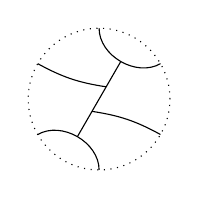
\begin{tikzpicture}[scale=0.9,baseline={([yshift=-3pt]current bounding box.center)}]
					\draw[dotted] (0,0) circle(1cm);
					\begin{scope}[yscale=1,xscale=-1]
					\draw (90:1cm) to [bend left=60] (150:1cm);
					\draw (210:1cm) to [bend left=10] (300:0.2cm);
					\draw (30:1cm) to [bend left=10] (120:0.2cm);
					\draw (120:0.61cm) to (300:0.61cm);
					\draw (270:1cm) to [bend left=60] (330:1cm);
					\end{scope}
				\end{tikzpicture}\ +\ 2\text{ rotations,} &
				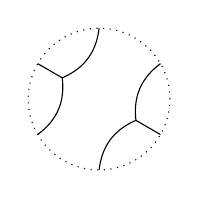
\begin{tikzpicture}[scale=0.9,baseline={([yshift=-3pt]current bounding box.center)}]
					\draw[dotted] (0,0) circle(1cm);
					\draw (150:1cm)  -- (150:0.6cm);
					\draw (90:1cm) to [bend left=30] (150:0.6cm);
					\draw (210:1cm) to [bend right=30] (150:0.6cm);
					\draw (330:1cm)  -- (330:0.6cm);
					\draw (270:1cm) to [bend left=30] (330:0.6cm);
					\draw (30:1cm) to [bend right=30] (330:0.6cm);
				\end{tikzpicture}\ +\ 2\text{ rotations,} &
				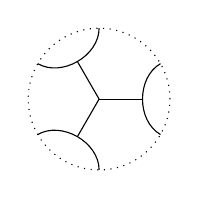
\begin{tikzpicture}[scale=0.9,baseline={([yshift=-3pt]current bounding box.center)}]
					\draw[dotted] (0,0) circle(1.cm);
					\draw (90:1cm) to [bend left=60] (150:1cm);
					\draw (210:1cm) to [bend left=60] (270:1cm);
					\draw (330:1cm) to [bend left=60] (30:1cm);
					\draw (0,0) to (120:0.61cm);
					\draw (0,0) to (240:0.61cm);
					\draw (0,0) to (0:0.61cm);
				\end{tikzpicture}\ +\ 1\text{ rotation}
			\end{tabular}
		\end{table}
	\noindent
	Because of $\dim(\mathfrak{C}_6)=37$, these diagrams obviously do not suffice to form a basis. Therefore, we will also take into account diagrams with one face of which there are seven (we will refer to the second diagram and its rotations as \emph{pentaforks}):
		\begin{table}[H]
			\begin{tabular}{cc}
				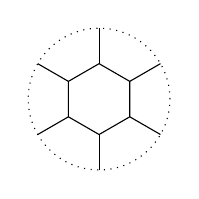
\begin{tikzpicture}[scale=0.9,baseline={([yshift=-3pt]current bounding box.center)}]
					\draw[dotted] (0,0) circle(1.cm);
					\draw (90:0.5cm) -- (150:0.5cm) -- (210:0.5cm) -- (270:0.5cm) -- (330:0.5cm) -- (30:0.5cm) -- cycle;
					\foreach \a in {30,90,...,330}
						\draw (\a:0.5cm) -- (\a:1cm);
				\end{tikzpicture}\ , &
				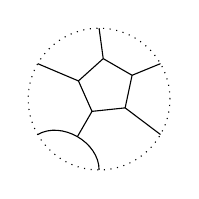
\begin{tikzpicture}[scale=0.9,baseline={([yshift=-3pt]current bounding box.center)}]
					\draw[dotted] (0,0) circle(1.cm);
					\draw (210:1cm) to [bend left=60] (270:1cm);
					\draw (240:0.2cm) -- (240:0.61cm);
					\begin{scope}[scale=0.8,shift={(60:0.25)}]
						\draw (240:0.5) -- (312:0.5) -- (24:0.5) -- (96:0.5) -- (168:0.5) -- cycle;
					\end{scope}
					\draw (330:1cm) to ([scale=0.8,shift={(60:0.25)}]312:0.5);
					\draw (30:1cm) to ([scale=0.8,shift={(60:0.25)}]24:0.5);
					\draw (90:1cm) to ([scale=0.8,shift={(60:0.25)}]96:0.5);
					\draw (150:1cm) to ([scale=0.8,shift={(60:0.25)}]168:0.5);
				\end{tikzpicture}\ +\ 5\text{ rotations}
			\end{tabular}
		\end{table}
	\noindent
%	and even the diagrams with two faces, which is only one:
%		\begin{table}[H]
%			\begin{tabular}{c}
%				\begin{tikzpicture}[scale=0.9,baseline={([yshift=-3pt]current bounding box.center)}]
%					\draw[dotted] (0,0) circle(1.cm);
%					\shade[ball color = red, opacity = 0.8] (0,0) circle (0.05cm);
%					\begin{scope}[scale=0.5,shift={(0,0.55)}]
%						\draw (90:0.7) -- (18:0.7) -- (306:0.7) -- (234:0.7) -- (162:0.7) -- cycle;
%					\end{scope}
%					\begin{scope}[yscale=-0.5,xscale=0.5,shift={(0,0.55)}]
%						\draw (234:0.7) -- (162:0.7) -- (90:0.7) -- (18:0.7) -- (306:0.7);
%					\end{scope}
%					\draw (90:1) -- ([scale=0.5,shift={(0,0.55)}]90:0.7);
%					\draw (150:1) -- ([scale=0.5,shift={(0,0.55)}]162:0.7);
%					\draw (30:1) -- ([scale=0.5,shift={(0,0.55)}]18:0.7);
%					\draw (210:1) -- ([yscale=-0.5,xscale=0.5,shift={(0,0.55)}]162:0.7);
%					\draw (270:1) -- ([yscale=-0.5,xscale=0.5,shift={(0,0.55)}]90:0.7);
%					\draw (330:1) -- ([yscale=-0.5,xscale=0.5,shift={(0,0.55)}]18:0.7);
%				\end{tikzpicture}\ +\ 2\text{ rotations}
%			\end{tabular}
%		\end{table}
	We now have $41$ candidate diagrams for a basis of dimension $37$. It turns out that leaving out any four of the six pentaforks yields a linear independent set of diagrams (see \cite[Proof of Proposition 6.4]{Morrison2017}) and we also know that this set of diagrams spans $\mathfrak{C}_6$ (see \cite[Lemma 6.25]{Morrison2017}), hence they form a basis of $\mathfrak{C}_6$.
	
	These are the vector spaces where almost all our calculations will take place. Later, we will see how to construct orthonormal bases for them in a canonical way, but for that purpose we will need the full category and not only its trivalent description.
	